%!TEX root = thesis.tex
\chapter{Implementation} \label{ch:implement}


% Framework
%     Loads ptx files
%     Memory limitations
%     Other programs have inefficient layers (cyclone)
%     Other open source programs dont have undo
%     Save and load project files
%     Speed up development through auto reload plugin architecture

\section{Layers and selections}
In order to segment a point cloud, one needs to be able to group sets of points. To promote ease of use we decided to adopt a system of selections and layers as is prevalent in many image and point cloud editing programs. Selections are used to temporarily select points and layers are used to manage more than one selection.

While traditional systems only support binary selections, our system supports 8 color selections. This is achieved through a 8 bit mask annotation attached to each point. The reason for eight color selections are two fold. Firstly a byte the smallest attribute that OpenGL lets one attach to a shader. Secondly, its useful to have more than one type of select when labeling point for use in classification algorithms. A larger number of selection colors would consume memory that has no foreseeable use. Managing an arbitrary number of point sets is what we designed layers for.

Beyond managing an arbitrary amount of point sets, it was thought useful \todo{This sounds a bit willy nilly...} to support set operations between layers. In this way, the results from different segmentations can be combined. E.g, if one has a crudely selected wall and meticulously segmented tree against the wall, one can remove tree points from the wall by subtracting the tree layer from the wall layer.

In order to support effective manipulation of multiple concurrently loaded point clouds, it was also necessary to cater layers that spanned more than one point cloud.

It was reported by our collaborators that the Cyclone \todo{Need source?} point cloud editing tool used excessive memory when creating many layers. Due to the propriety nature of the software we can only speculate as to the reason. It was however a design goal to make layer creation cheap. 

A naive approach to layer creation would be simply create a vector and fill it with indices corresponding to the points in the set. However this would lead to a linear increase in memory consumption as the number of points in layers grew. This is likely how Cyclone was implemented. It would also lead to $O(n^{2})$ set operations and manging indices from multiple clouds with such a data structure would be difficult.

Our approach is to add a numerical label to each point in a cloud and then keep a separate data structure that maps a label to its associate layers.

% One can thus determine what layers a point belongs to by looking up its label, then seeing what layers are mapped to that label.

In this scheme, each point initially carries a 0 label that doesn't map to a layer. When the first layer set is created, the points in that set are labeled with 1. An entry is then created associating the new layer with the label 1 (see figure~\ref{fig:layer2}).

When a second layer is created, the points in that layer are labeled with the next available integer label (see figure~\ref{fig:layer3}).

If a layer is created that contain points already in another layer, the newly labeled points will simply get the next available label. Overlapping points however need to be relabeled with the next available label. The label associated with with the overlapping points is then assigned to both the old layer and the new layer (see figure~\ref{fig:layer4}).


\begin{figure}[ht]
	\begin{minipage}[b]{\linewidth}
		\centering
		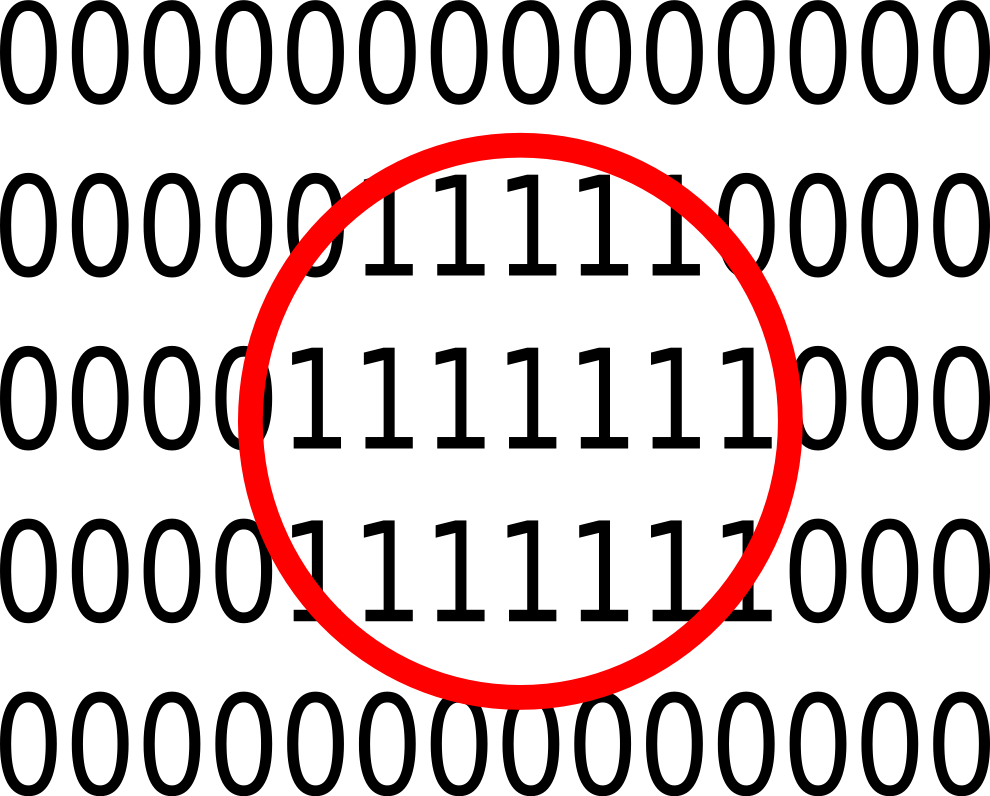
\includegraphics[width=0.45\textwidth]{images/layers2}
	\end{minipage}
	\\\\
	\begin{minipage}[b]{0.48\linewidth}
		\hfill
		\begin{tabular}[b]{|l|l|l|l|}
			\hline
			Layer & Labels \\
			\hline
			\textcolor{red}{red}       & 1 \\
			\hline
		\end{tabular}
	\end{minipage}
	\hspace{0.5cm}
	\begin{minipage}[b]{0.5\linewidth}
		\begin{tabular}[b]{|l|l|l|l|}
			\hline
			Label & Layers \\
			\hline
			1       & \textcolor{red}{red} \\
			\hline
		\end{tabular}
		\hfill
	\end{minipage}
	\caption{One layer\label{fig:layer2}}
\end{figure}



\begin{figure}[ht]
	\begin{minipage}[b]{\linewidth}
		\centering
		\includegraphics[width=0.45\textwidth]{images/layers3}
	\end{minipage}
	\\\\
	\begin{minipage}[b]{0.48\linewidth}
		\hfill
		\begin{tabular}[b]{|l|l|l|l|}
			\hline
			Layer & Labels \\
			\hline
			\textcolor{red}{red}       & 1 \\
			\textcolor{green}{green}       & 2 \\
			\hline
		\end{tabular}
	\end{minipage}
	\hspace{0.5cm}
	\begin{minipage}[b]{0.5\linewidth}
		\begin{tabular}[b]{|l|l|l|l|}
			\hline
			Label & Layers \\
			\hline
			1       & \textcolor{red}{red} \\
			2       & \textcolor{green}{green} \\
			\hline
		\end{tabular}
		\hfill
	\end{minipage}
	\caption{Two non overlapping layers\label{fig:layer3}}
\end{figure}

\begin{figure}[ht]
	\begin{minipage}[b]{\linewidth}
		\centering
		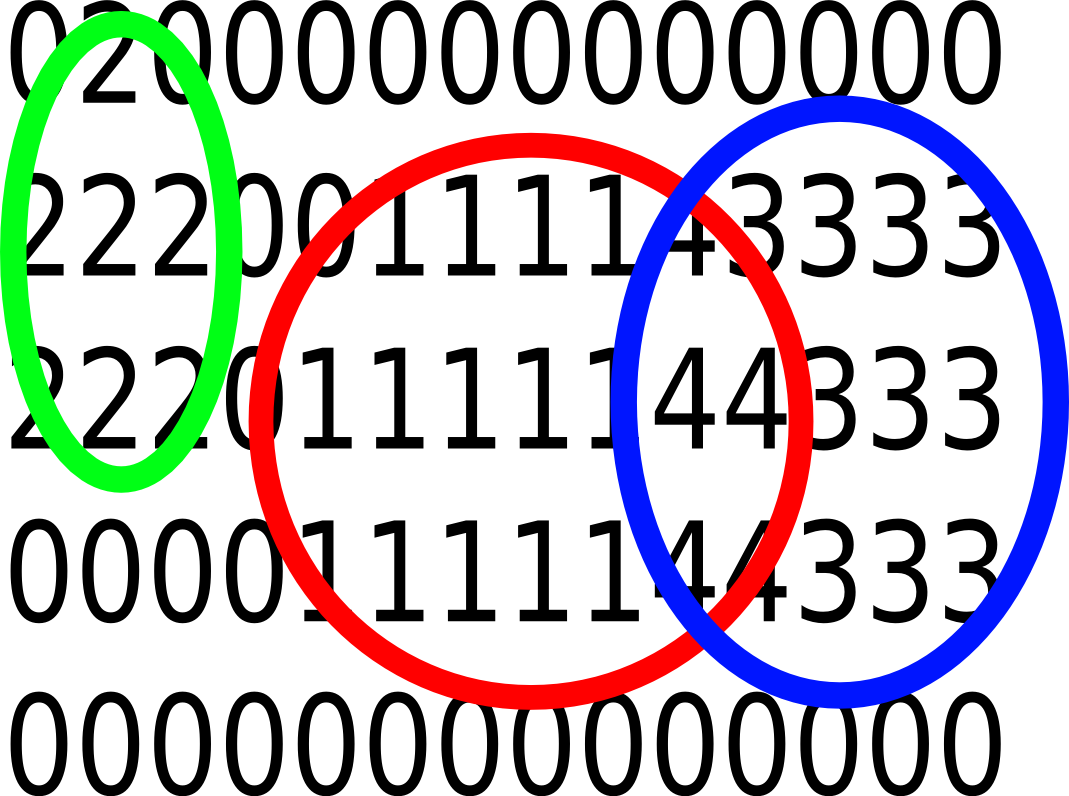
\includegraphics[width=0.45\textwidth]{images/layers4}
	\end{minipage}
	\\\\
	\begin{minipage}[b]{0.46\linewidth}
		\hfill
		\begin{tabular}[b]{|l|l|l|l|}
			\hline
			Layer & Labels \\
			\hline
			\textcolor{red}{red}       & 1, 4 \\
			\textcolor{green}{green}       & 2 \\
			\textcolor{blue}{blue}       & 3, 4 \\
			\hline
		\end{tabular}
	\end{minipage}
	\hspace{0.5cm}
	\begin{minipage}[b]{0.5\linewidth}
		\begin{tabular}[b]{|l|l|l|l|}
			\hline
			Label & Layers \\
			\hline
			1       & \textcolor{red}{red} \\
			2       & \textcolor{green}{green} \\
			3       & \textcolor{blue}{blue} \\
			4       & \textcolor{blue}{blue}, \textcolor{red}{red} \\
			\hline
		\end{tabular}
		\hfill
	\end{minipage}
	\caption{Three layers with one overlap\label{fig:layer4}}
\end{figure}


Our approach has several advantaged over the naive approach. Firstly, creating new layers is memory efficient. Set operations between layers are extremely cheap computationally as only the table that maps labels to layers need to manipulated. Alpha blending overlapping layers during rendering is also extremely efficient and allows for visual comparisons between layers to be performed.

This approach however, can quickly exhaust the available labels should high overlapping between layers occur. The worse scenario is that each newly created layer overlaps with ever other existing label. Should this happen, the number of bits allocated for the label will be the maximum number of layers. For our implementation that is 16 layers. This is however not considered to be a likely scenario. Should no overlapping occur one could have 65536 with 16 bits. The number of layers one an accommodate is equivalent to $2^b/i$ where $b$ is the number of bits used for a label and $i$ i the number of average intersections each layer is expected to have with other layers \todo{Questionable math, needs review}.



\begin{table}[ht]
	\begin{center}
	\begin{tabular}{|l|l|l|l|}
	\hline
	Index & X,Y,Z,I (float{[}4{]}) & Label buffer (uint16) & Selection mask (uint8)\\
	\hline
	0     & 0.8, 1.2, 0.2, 0.9 & 0                     & 10000000               \\
	1     & 0.7, 0.5, 0.8, 0.3 & 2                     & 10000000               \\
	2     & 4.3, 0.5, 1.7, 0.9 & 2                     & 10000000               \\
	3     & 0.6, 1.8, 0.1, 0.6 & 1                     & 01000000               \\
	4     & 0.9, 0.5, 0.8, 0.5 & 2                     & 01000000               \\
	5     & 0.1, 0.4, 3.2, 0.9 & 3                     & 01000000               \\
	6     & 2.2, 0.5, 0.3, 0.2 & 5                     & 00000000               \\
	7     & 1.0, 0.9, 0.1, 0.5 & 4                     & 00000000               \\
	\vdots     & \vdots & \vdots  & \vdots             \\
	\hline
	\end{tabular}
	\end{center}
	\caption{GPU point cloud buffer layout}
\end{table}


\begin{table}[ht]
	\begin{center}
	\begin{tabular}{|l|l|l|l|}
	\hline
	Layer  name & Color    & Visible & Labels \\
	\hline
	grass       & \#009900 & true & 0, 2, 4      \\
	walls       & \#0000FF & true & 0, 3  \\
	tree        & \#00FF00 & false & 2, 3   \\
	\vdots     & \vdots & \vdots   & \vdots          \\
	\hline
	\end{tabular}
	\end{center}
	\caption{Layer data structure}
\end{table}


\begin{table}[ht]
	\begin{center}
	\begin{tabular}{|l|l|l|}
	\hline
	Label & Color  \\
	\hline
	0       & walls.color \\
	1       & grass.color \\
	3       & mix(walls.color, tree.color)	\\
	4       & grass.color	\\
	\vdots     & \vdots      \\
	\hline
	\end{tabular}
	\end{center}
	\caption{GPU label color table}
\end{table}


\section{Undo}
QT based stack